\section{Utilizzo applicazione}
	\subsection{Aggiunta dei dati di addestramento}
	Per aggiungere i dati di addestramento, cliccare sul pulsante "Seleziona un file csv".
	\begin{figure}[H] 	
		\begin{center}
			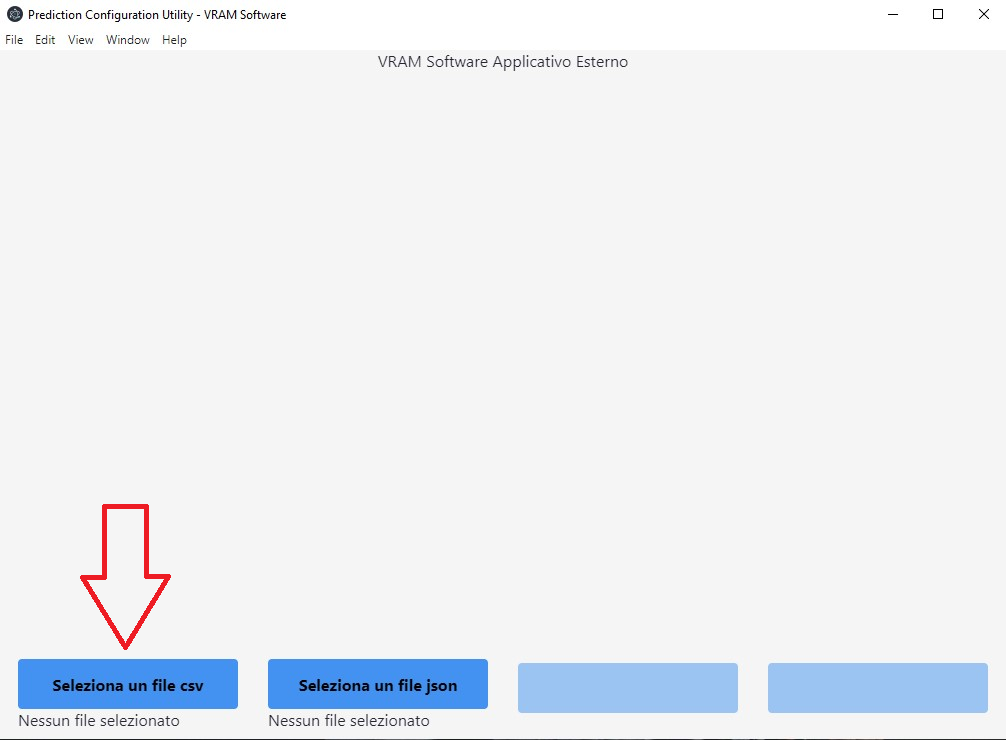
\includegraphics[width=\linewidth]{img/1.png}
		\end{center}
		\caption{Seleziona file csv}	
	\end{figure}
	Si aprirà il file manager di sistema e sarà possibile importare il file desiderato. Una volta selezionato, apparirà un pop-up dove sarà possibile scegliere l'algoritmo di predizione che si desidera addestrare per quei dati e selezionare l'ordine dei predittori. L'ultimo selezionato sarà il predetto.
	\begin{figure}[H] 	
		\begin{center}
			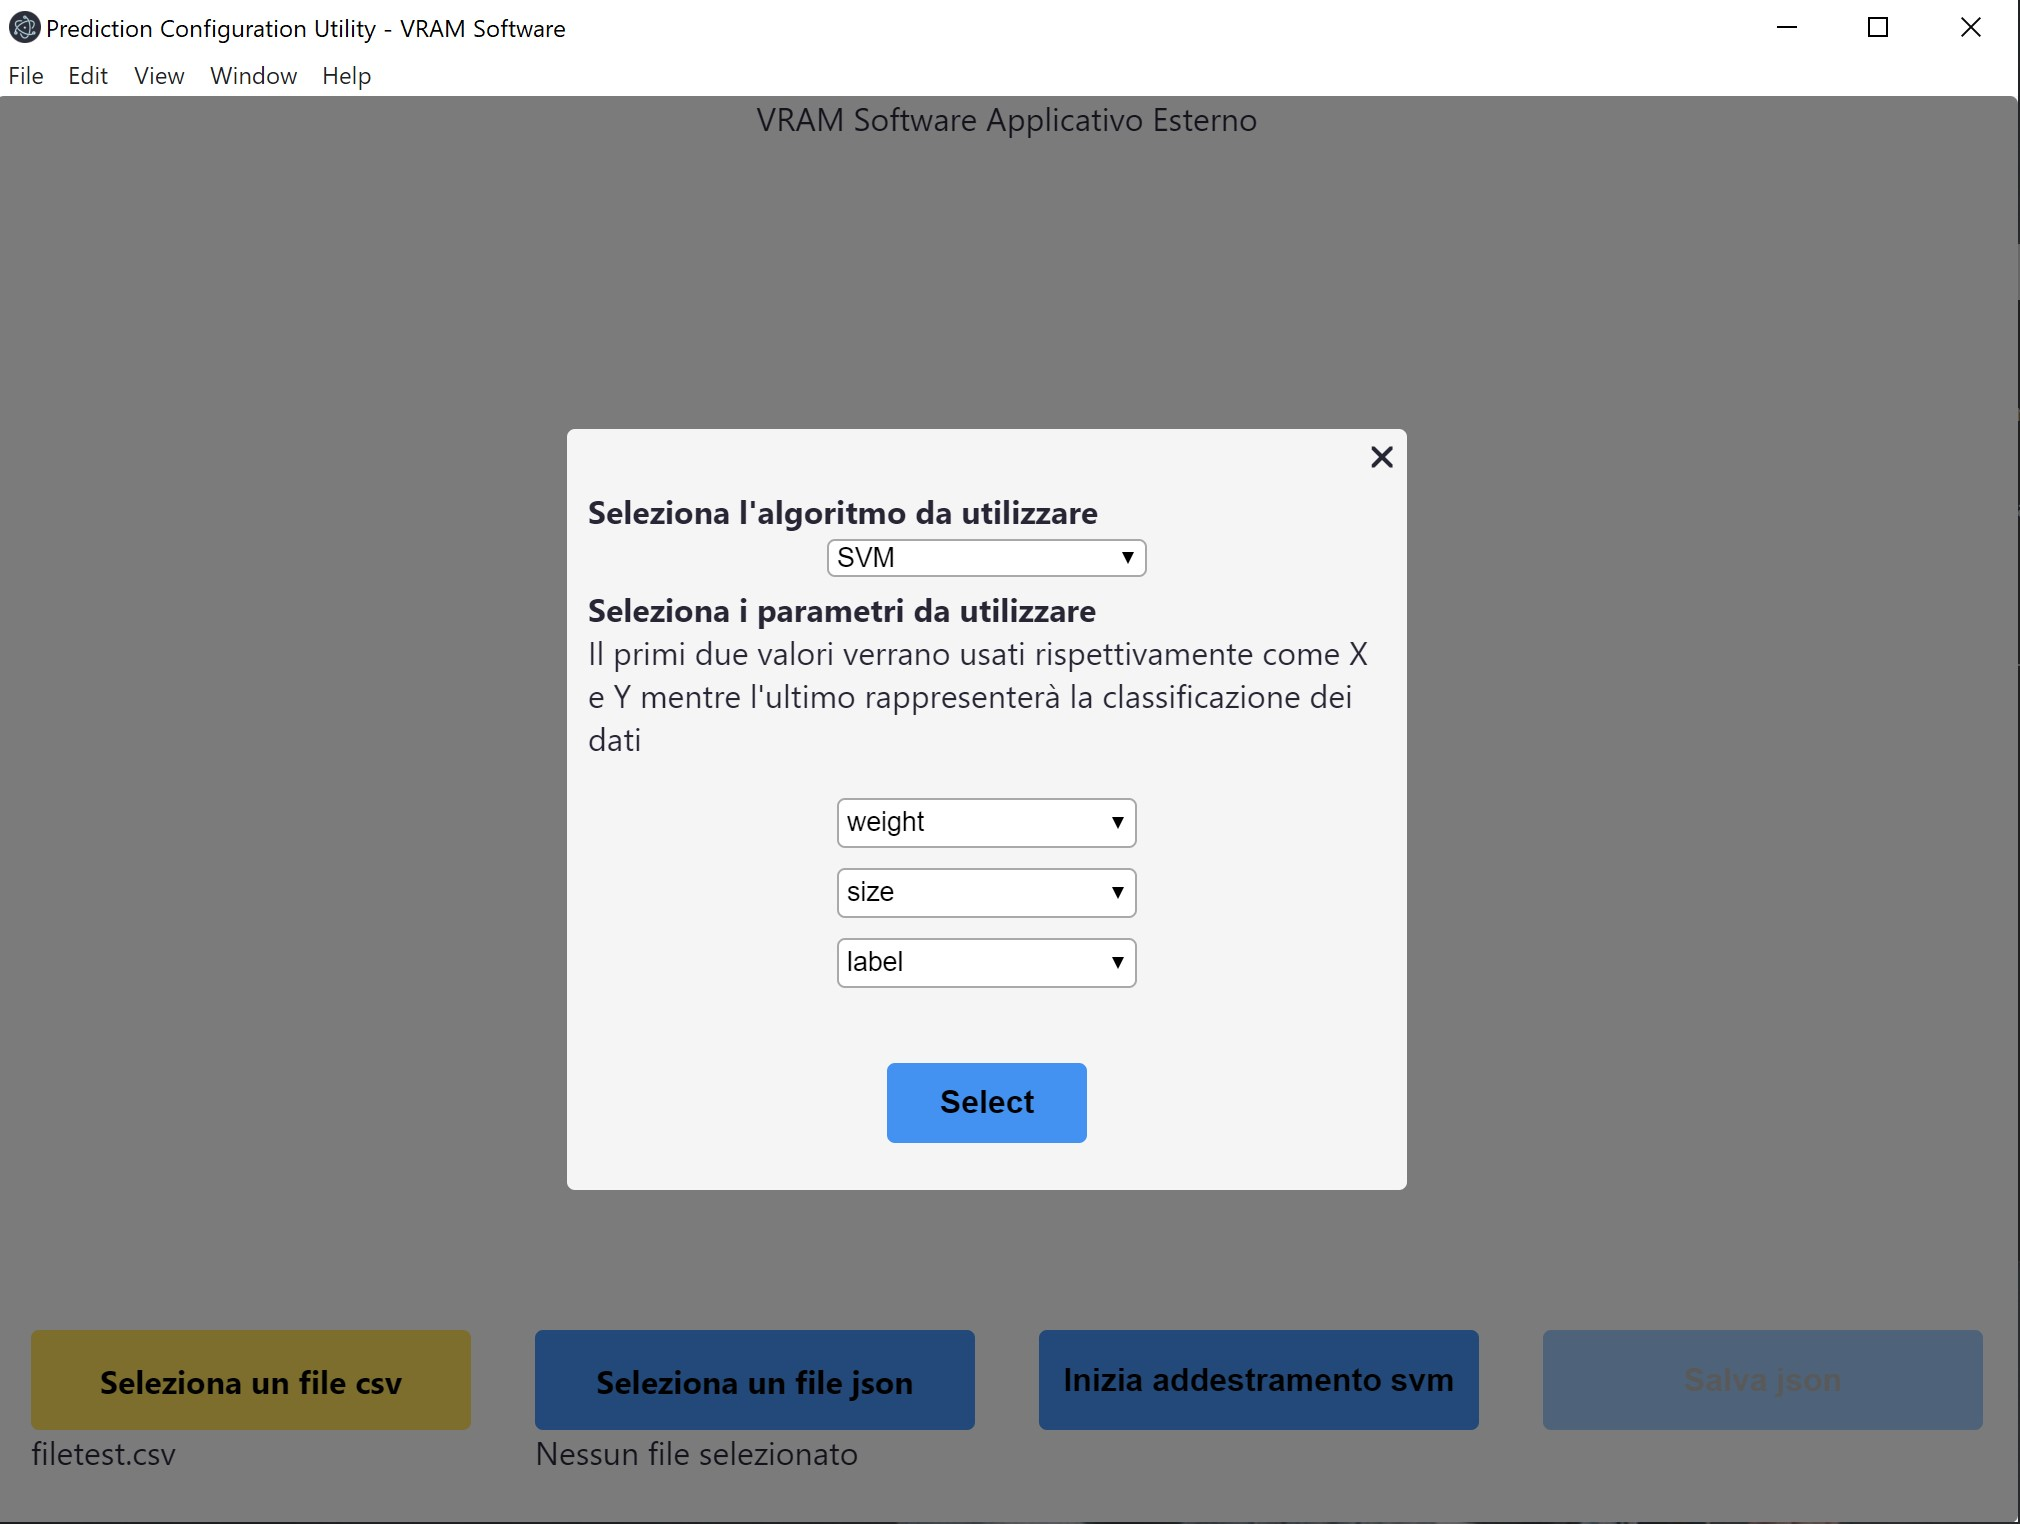
\includegraphics[width=\linewidth]{img/2.jpg}
		\end{center}
		\caption{Selezione dell'algoritmo e dei parametri di predizione}	
	\end{figure}
	Una volta selezionati apparirà un grafico in base all'ordine scelto.
	\subsection{Aggiunta di un file di configurazione}
	Per aggiungere un file di configurazione precedentemente creato, cliccare sul pulsante "Seleziona un file json".
	Si aprirà il file manager di sistema e sarà possibile importare il file desiderato. Una volta selezionato verranno automaticamente caricate e aggiornate le note dell'addestramento.
	\begin{figure}[H] 	
		\begin{center}
			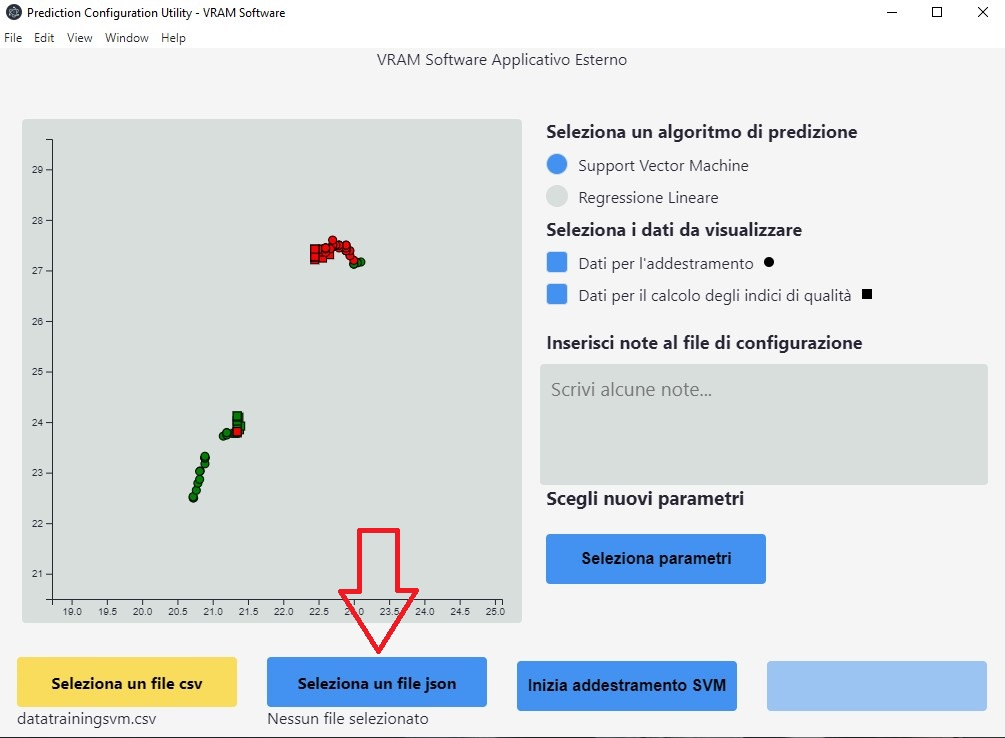
\includegraphics[width=\linewidth]{img/3.jpg}
		\end{center}
		\caption{Seleziona file Json}	
	\end{figure}
	\subsection{Avvio dell'addestramento}
	Una volta aggiunti i dati di addestramento sarà possibile cliccare sul pulsante "Avvio addestramento". Al termine dell'addestramento verrà visualizzato il messaggio "Addestramento avvenuto" e, se le dimensioni dei dati lo consentono, il risultato sarà visualizzabile nel grafico. Verranno inoltre visualizzati gli indici di qualità all'interno di un riquadro con un colore dipendente dalla bontà dell'addestramento:
	\begin{itemize}
		\item \textbf{verde} se l'indice è superiore al 60\%;
		\item \textbf{giallo} se l'indice compreso tra il 40\% e il 60\%;
		\item \textbf{rosso} se l'indice è inferiore al 40\%.
	\end{itemize}
	\begin{figure}[H] 	
		\begin{center}
			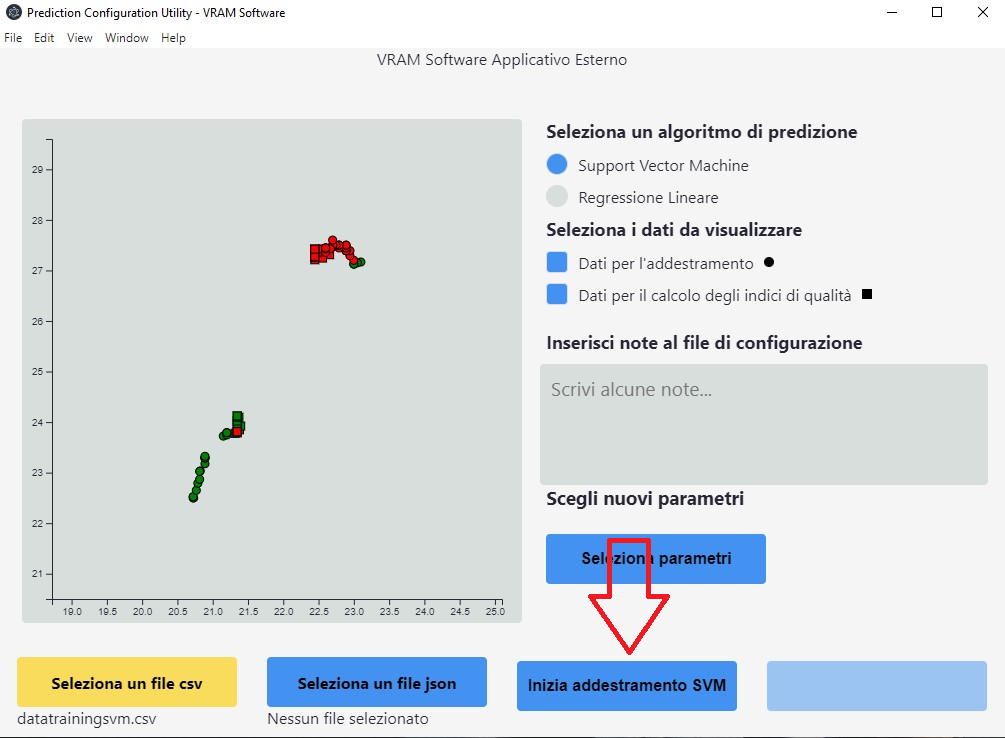
\includegraphics[width=\linewidth]{img/4.png}
		\end{center}
		\caption{Avvio dell'addestramento}	
	\end{figure}
	\begin{figure}[H] 	
		\begin{center}
			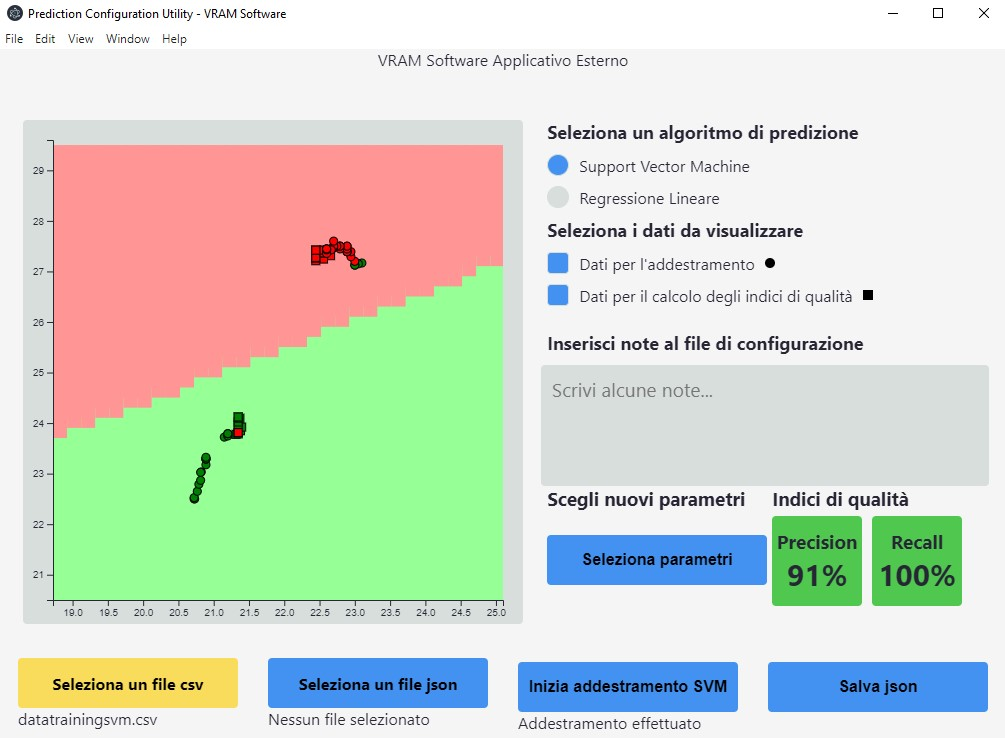
\includegraphics[width=\linewidth]{img/4.jpg}
		\end{center}
		\caption{Addestramento avvenuto}	
	\end{figure}
	
	\subsection{Selezione dati da visualizzare nel grafico}
	In qualsiasi momento è possibile selezionare i dati da visualizzare sul grafico: solo i dati utilizzati per l'addestramento, solo i dati utilizzati per il calcolo degli indici di qualità o entrambi. I primi saranno rappresentati con un cerchio, i secondi con un quadrato.
	\begin{figure}[H] 	
		\begin{center}
			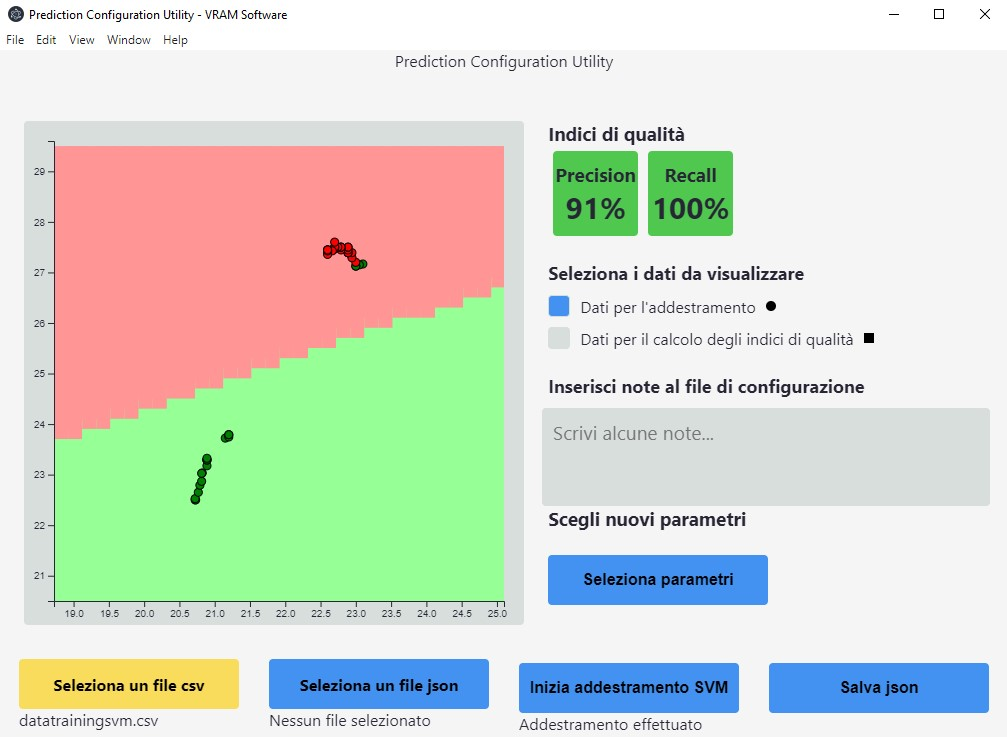
\includegraphics[width=\linewidth]{img/6.jpg}
		\end{center}
		\caption{Visualizzazione dati addestramento}	
	\end{figure}
	\begin{figure}[H] 	
		\begin{center}
			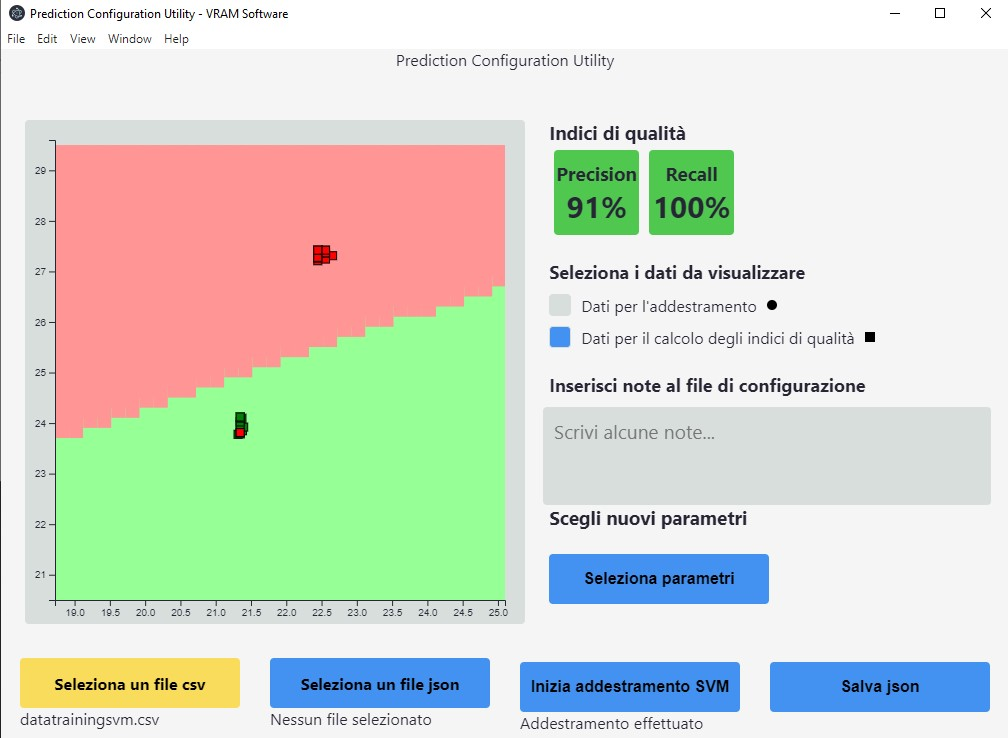
\includegraphics[width=\linewidth]{img/8.jpg}
		\end{center}
		\caption{Visualizzazione dati indici di qualità}	
	\end{figure}

	\subsection{Aggiunta di note all'addestramento}
	In qualsiasi momento è possibile aggiungere delle note all'addestramento tramite l'apposito box. Queste saranno aggiunte al file json prodotto in seguito all'addestramento.
	\begin{figure}[H] 	
		\begin{center}
			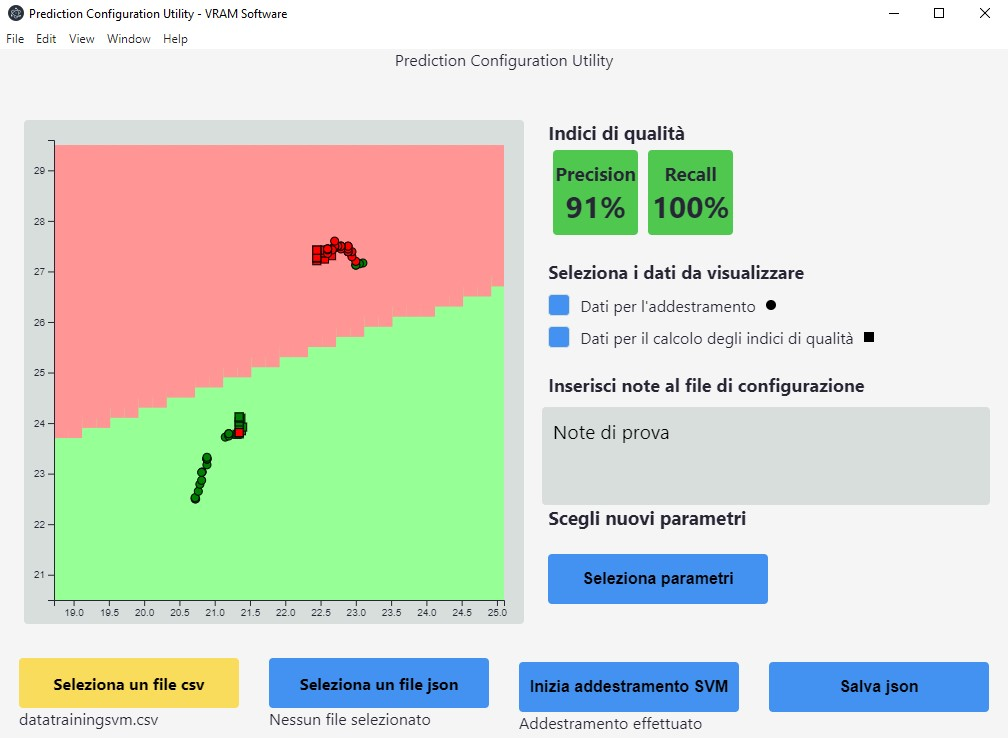
\includegraphics[width=\linewidth]{img/7.jpg}
		\end{center}
		\caption{Inserimento delle note}	
	\end{figure}
		
	\subsection{Cambio dei parametri}
	Cliccando sul pulsante "Cambia parametri" apparirà un pop-up dove sarà possibile cambiare il predetto e l'ordine dei predittori, come avviene nell'inserimento del file.
	\begin{figure}[H] 	
		\begin{center}
			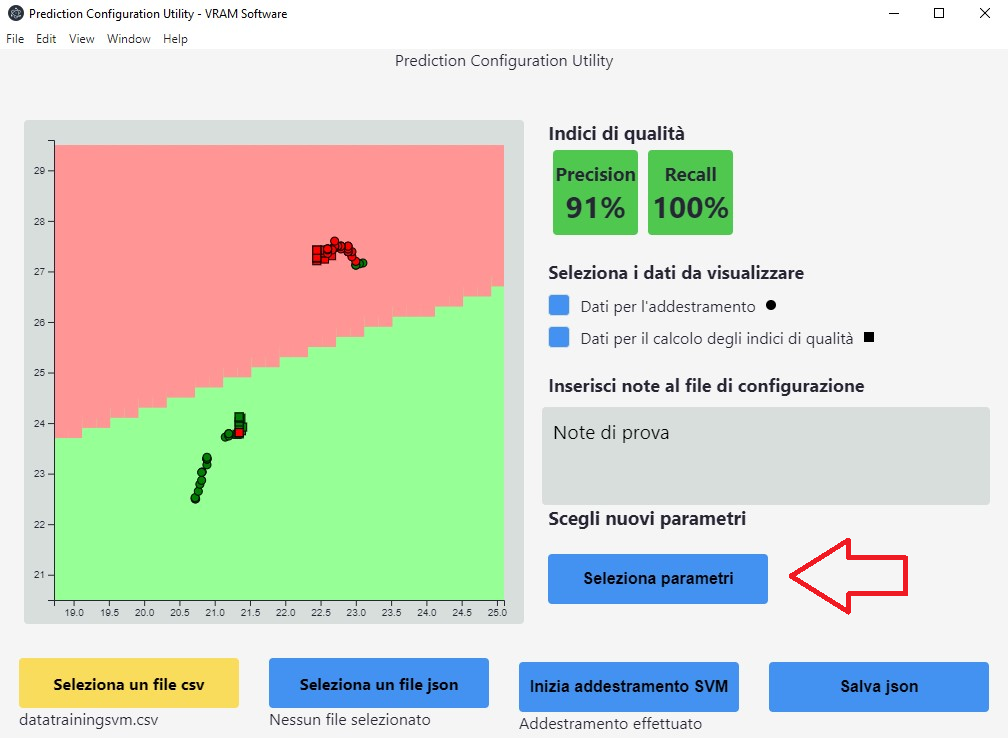
\includegraphics[width=\linewidth]{img/9.jpg}
		\end{center}
		\caption{Cambio dei parametri di addestramento}	
	\end{figure}
	\subsection{Salvataggio dei risultati}
	Cliccando sul pulsante "Salva json" apparirà un pop-up in cui si potrà inserire il nome del file e selezionare la cartella in cui lo si vuole salvare. Questo file conterrà tutte le informazioni dell'addestramento necessarie per eseguire la predizione, comprese le eventuali note scritte nel box dell'applicazione.
	\begin{figure}[H] 	
		\begin{center}
			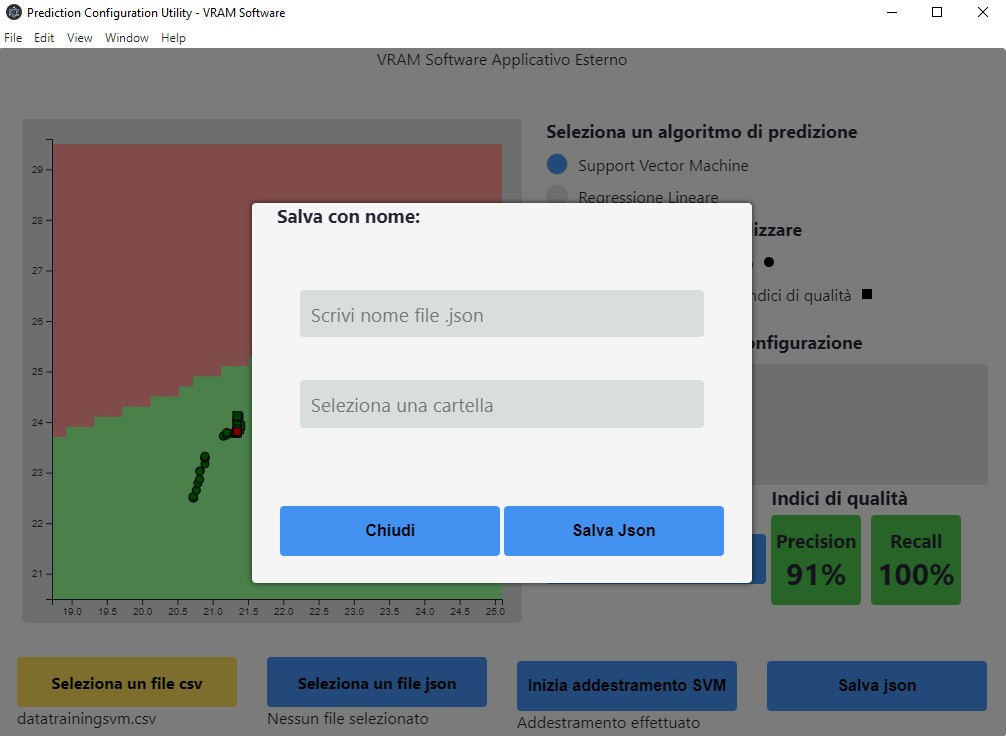
\includegraphics[width=\linewidth]{img/10.jpg}
		\end{center}
		\caption{Salva file Json}	
	\end{figure}
	
